\documentclass[twocolumn]{revtex4-2}
\usepackage[spanish]{babel}
\usepackage{}
\usepackage{hyperref}
\usepackage{xurl}
\usepackage{float}
\usepackage{graphicx}
\usepackage{dcolumn}
\usepackage{bm}
\usepackage{textcomp}
\usepackage{float}
\usepackage{graphicx}   % Para incluir imágenes
\usepackage{caption} 
\usepackage{subcaption}
\usepackage[utf8]{inputenc}% Para personalizar captions
\usepackage{url}
\usepackage{float} % en el preámbulo
\usepackage[spanish, es-tabla, es-punto]{babel}
\usepackage{xcolor}
\usepackage{minted}
\includegraphics[width=0.7\textwidth]{...}
\setminted{
    fontsize=\footnotesize,
    frame=single,
    breaklines=true,       % Permite cortar líneas largas
    breakanywhere=true,    % Corta en cualquier punto si es necesario
    tabsize=2
}
\captionsetup[figure]{skip=0pt} % Quita el espacio entre imagen y título
\begin{document}
\spanishdecimal{.}
\title{}
\author{Jesús Armando Cañas}
\author{Miguel Angel Perdomo}

\date{\today}


\begin{abstract}
\vspace{-0.5cm}
\end{abstract}

\maketitle

\section{Introducción}
\begingroup
\vspace{-0.3cm}


\section{Marco teórico}
\subsection{Test de Chi cuadrado $\chi$ }
\subsection{Mínimos cuadrados}
\subsection{Diodos}
\subsubsection{semiconductores}
Los semiconductores son elementos cuyas propiedades conductivas oscilan entre las de un elemento conductor y un aislante. Por lo general, hay dos tipos de materiales semiconductores: un solo cristal y compuesto. Los semiconductores de un solo
cristal como el germanio (Ge) y el silicio (Si) tienen una
estructura cristalina repetitiva, en tanto que compuestos como
el arseniuro de galio (GaAs), el sulfuro de cadmio (CdS), el ni
truro de galio (GaN) y el fosfuro de galio y arsénico (GaAsP)
se componen de dos o más materiales semiconductores de
diferentes estructuras atómicas. ~\cite{rosadio}

\subsubsection{Clasificación de los semiconductores}
Los semiconductores se clasifican en dos tipos:
\begin{enumerate}
    \item \textbf{Semiconductor tipo n}: son los semiconductores en los que hay un exceso de electrones libres comparados con el número de huecos. Es por esto que se le atribuye el nombre $n$, por el carácter negativo. ~\cite{rosadio}
    \item \textbf{Semiconductores tipo p:} en este tipo de semiconductores hay un exceso de huecos comparado con el número de electrones libres. Los elementos más utilizados para este propósito son el boro, galio e indio. El término p se atribuye refiriéndose al positivo. ~\cite{rosadio}
    
\end{enumerate}
\subsubsection{Unión p-n, composición del diodo}
Cuando se dopa un material semiconductor de modo que una mitad sea tipo p y la otra de tipo n, se forma lo que denominamos un diodo $semiconductor$ y el borde entre la zona de tipo p y la zona de tipo n se denomina unión p-n. ~\cite{rosadio}

\subsubsection{Clasificación de los tipos de diodo}
\begin{itemize}
    \item \textbf{Polarización directa}\newline Un diodo tiene polarización directa cuando se conecta un terminal positivo al material de tipo p y un material negativo al material de tipo n tal como se muestra en la imagen \ref{directa}. \newline
    \begin{figure}
        \centering
        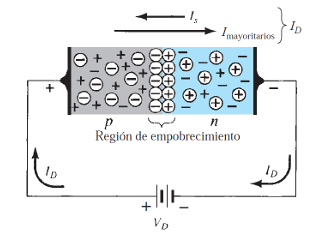
\includegraphics[width=1\linewidth]{Imagenes/diodo con polarizacion directa.png}
        \caption{Diodo con polarización directa}
        \label{directa}
    \end{figure}
    En este caso de polarización directa, los electrones y huecos
    son empujados hacia la unión. Si la tensión entre las termi
    nales es menor que la barrera de potencial, los electrones
    libres de la zona n no tienen la suficiente energía para atravesar
    la zona de deplexión. Cuando entran en esta zona, los iones se
    ven empujados de vuelta a la región n, por lo que no circula
    corriente a través del diodo.
    Cuando la tensión entre las terminales es mayor que
    la barrera de potencial, se empuja de nuevo a huecos y
    electrones libres hacia la unión. En este caso, existe un flujo de electrones de la parte de material n a la parte de material p.

    ~\cite{rosadio}
    
    \item \textbf{Polarización inversa}\newline Un diodo tiene polarización inversa si se le conecta una terminal negativa a la parte del material tipo n como se muestra en la imagen\ref{inversa}.

    Aquí los huecos son atraídos por el material negativo mientras que los electrones libres son atraídos por el positivo. Esto
    origina que los electrones libres y huecos se alejen de la unión
    y a medida que se alejan, dejan tras su paso a iones positivos y
    negativos respectivamente, originando un ensanchamiento de
    Figura 2. Diodo con polarización inversa
    la zona de deplexión la cual crea una barrera demasiado grande
    para que los portadores mayoritarios la puedan superar, por lo
    que el flujo de portadores mayoritarios se reduce a cero. Sin
    embargo, el número de portadores minoritarios que entran a
    la zona de deplexión no cambia, y se producen vectores de
    flujo de portadores minoritarios de la misma magnitud. ~\cite{rosadio}

    La corriente en la polarización inversa se denomina corriente de $ saturación$, el término saturación se deriva del hecho de que no cambia significativamente con los cambios de potencial proporcionados al circuito eléctrico.
    
    \begin{figure}[H]
        \centering
        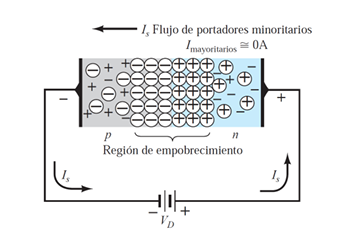
\includegraphics[width=1\linewidth]{Imagenes/diodo con polarizacion inversa.png}
        \caption{Diodo con polarización inversa}
        \label{inversa}
    \end{figure}
\end{itemize}


\subsection{Relación de la constante de Boltzmann en circuitos con diodos}

En los circuitos con diodos, la constante de Boltzmann $k_B$ juega un papel fundamental en la descripción del transporte de carga, particularmente en la ecuación característica corriente-voltaje  del diodo.

La corriente en un diodo de unión p-n está dada por:

\begin{equation}
I = I_s \left( e^{\frac{qV}{\eta k_B T}} - 1 \right)
\end{equation}

donde:
\begin{itemize}
    \item $I_s$ es la corriente de saturación,
    \item $q$ es la carga del electrón,
    \item $V$ es el voltaje aplicado,
    \item $\eta$ es el coeficiente de idealidad,
    \item $k_B$ es la constante de Boltzmann,
    \item $T$ es la temperatura absoluta.
\end{itemize}

La constante de Boltzmann aparece a través del denominado \textbf{voltaje térmico}, definido como:

\begin{equation}
V_T = \frac{k_B T}{q}
\end{equation}

Este voltaje térmico determina la escala a la cual la temperatura afecta el comportamiento del diodo. A temperatura ambiente ($T \approx 300\,K$) ~\cite{leon2014}, su valor es aproximadamente:

\begin{equation}
V_T \approx 25.9 \, \text{mV}
\end{equation}

\subsubsection{Interpretación física}

La presencia de $k_B$ en la ecuación del diodo refleja que el transporte de portadores está gobernado por procesos térmicos. Específicamente:

\begin{itemize}
    \item Controla la energía térmica disponible para que los electrones superen la barrera de potencial.
    \item Determina la generación de portadores minoritarios.
    \item Influye en la corriente de saturación y en la conducción en polarización inversa.
\end{itemize}

\subsubsection{Importancia en circuitos electrónicos}

En circuitos con diodos, la constante de Boltzmann afecta:

\begin{itemize}
    \item La pendiente de la curva IV (sensibilidad del diodo).
    \item El comportamiento con la temperatura.
    \item El diseño de circuitos analógicos como rectificadores y detectores.
\end{itemize}

Por lo tanto, $k_B$ conecta directamente la física estadística con el funcionamiento macroscópico de los dispositivos electrónicos.
\subsection{Matriz de covarianza}



\section{Metodología}



\subsection{Procedimiento}
\section{Resultados}
\subsection{Medidas por intervalos de 0.01 V}
El ajuste obtenido para las medidas tomadas por intervalos de 0.01 V se muestra en la gráfica \ref{0.01}.

\begin{figure}[H]
    \centering
    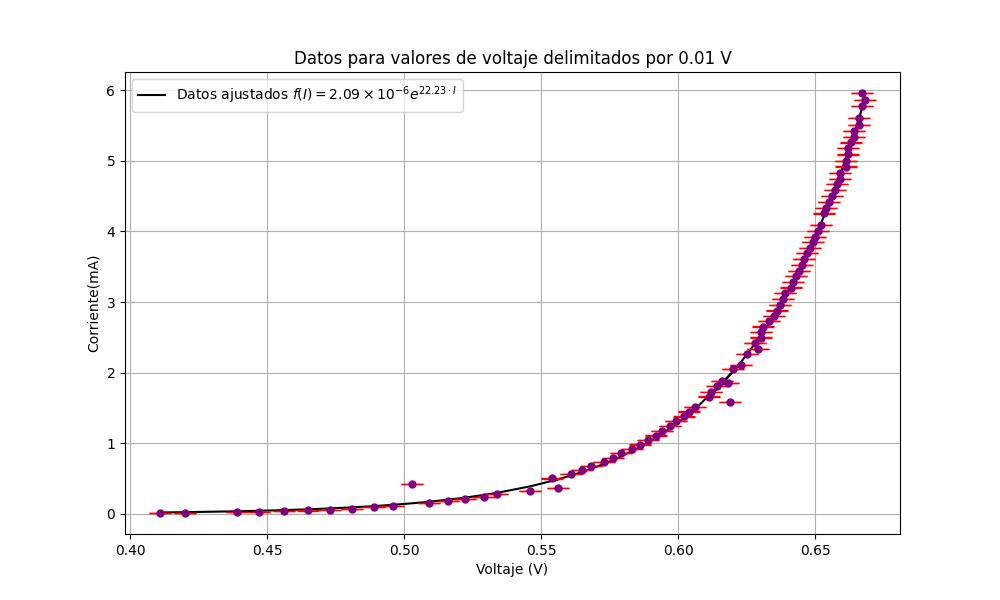
\includegraphics[width=1\linewidth]{Imagenes/datos_0.01.jpg}
    \caption{imagen correspondiente al ajuste exponencial para los datos tomados por intervalos de 0.01 V}
    \label{0.01}
\end{figure}
Usando el text de Chi cuadrado para comprobar la bondad del ajuste se llego a que el ajustes es bueno ya que se pudo refutar la hipótesis nula.

De la gráfica se puede deducir que para el ajuste exponencial de ecuación \ref{exponencial}
\begin{equation}
  f(x) = a e ^ {b x}
  \label{exponencial}
\end{equation}
Los valores de los parámetros ajustados con sus correspondientes errores estándares son los siguientes : 
$a = (2.0 \pm 0.2) \times 10 ^ {-6} \ y \ b = (22.2 \pm 0.2) $
. Usando el valor de $b$ para calcular la constante de Boltzman $K_b$ como se muestra en el marco teórico el valor obtenido es :
$K_b = 1.27 \times 10^{-23} $

Con un error porcentual de valor 

\subsection{Medidas por intervalos de 0.05}

En este caso, como fue indicado en la metodología, se linealizó la función exponencial modelo del sistema físico y luego se verificó la bondad del ajuste usando $R^2$ de la teória de mínimos cuadrados.
\begin{figure}[H]
    \centering
    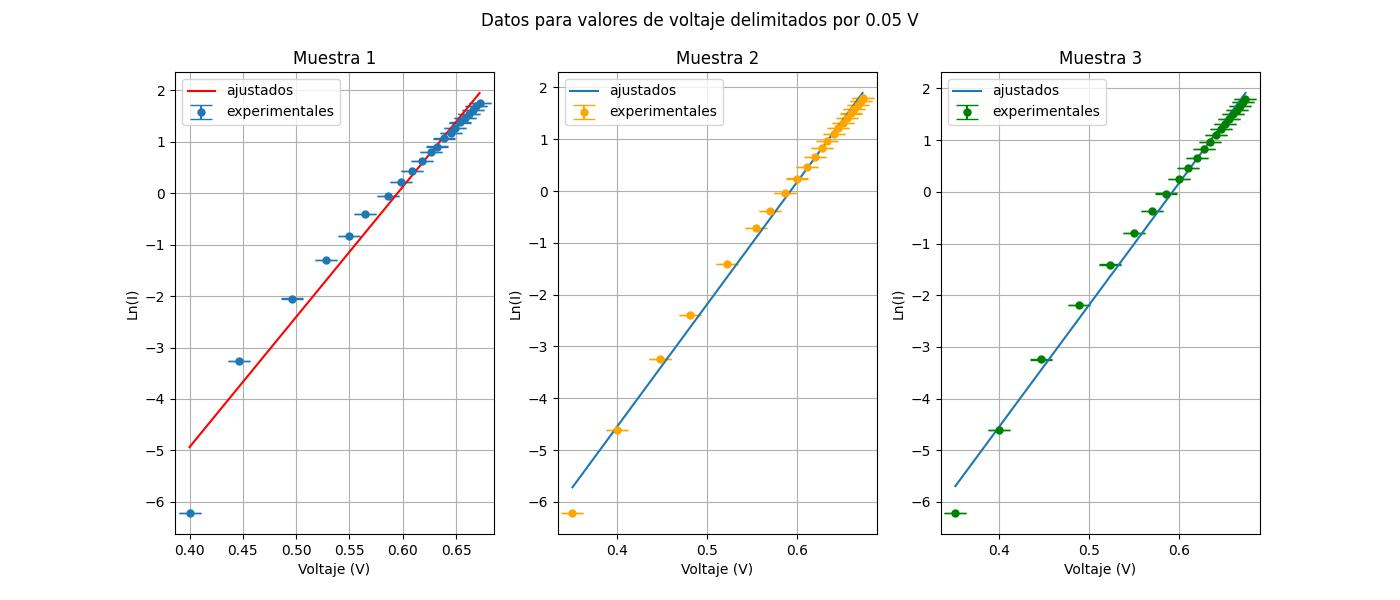
\includegraphics[width=1\linewidth]{Imagenes/datos_0.05.jpg}
    \caption{Gráficos obtenidos para la linealización de las medidas }
    \label{0.05}
\end{figure}

Los valores obtenidos de $R^2$ para los ajustes son $0.96 ,0.99,0.99$ respectivamente para cada una de las gráficas.

Por otro lado, los valores obtenidos de $K_b $ de los parámetros a de los ajustes son los siguientes: $1.2 \times 10^{-23}, 1.2 \times 10^{-23},1.2 \times 10^{-23}$ cuya incertidumbre estándar es insignificante.

\section{Conclusiones}
{\setlength{\parskip}{10pt}
}
\begin{enumerate}

\item
\end{enumerate}
\begin{thebibliography}{99}

\bibitem{rosadio}
G. Rosadio Vega, \emph{Circuitos básicos con diodos}. Lima, Perú: Universidad Nacional de Ingeniería, Departamento de Ingeniería Física, Facultad de Ciencias, s.f.

\bibitem{leon2014}
J. A. León Gil, \emph{Desarrollo de diodos túnel}. Apodaca, Nuevo León, México: Centro de Investigación en Materiales Avanzados, S.C., 2014.
\end{thebibliography}

\appendix


\end{document}









